\documentclass[10pt]{article}
\usepackage{icmlko}

\icmlmeta{IP 파운데이션 월드모델}{5}{옳은 축과 찾을 수 있는 축}{노트 4의 유의성은 선택 편향이었다 --- 그러나 다섯 축 자체는 살아남았다}

\begin{document}

\twocolumn[
\icmlheader

\begin{abstract}
노트 4는 다섯 개 속성이 처음으로 상수를 유의하게 이겼다고 보고했다(차이 $-$0.0540,
95\% 신뢰구간 $-$0.103에서 $-$0.010). 그 다섯은 열 개 후보 중에서 골랐는데, 고르는 데
쓴 데이터와 검정하는 데 쓴 데이터가 같았다. 이 노트는 그 편향을 중첩 교차검증으로
제거한다. \textbf{결과는 노트 4의 표제 주장을 철회시킨다.} 폴드 안에서 다섯을 새로
고르게 하면 차이는 $-$0.0400으로 줄고 신뢰구간이 0을 넘어간다. 그런데 같은 실험에서
예상 밖의 것이 살아남았다 --- \emph{선택을 아예 하지 않고 열 개를 전부 쓴 집합}은
유의하게 이긴다(차이 $-$0.0376, 신뢰구간 $-$0.0735에서 $-$0.0042). 표본 75건에서
선택은 도움이 아니라 해악이었다. 한편 IP 무작위 분할을 40회 반복하면 노트 4의 고정
다섯 종은 40회 전부 상수를 이긴다(100\%). 세 결과를 화해시키면 하나의 구분이 남는다:
\textbf{그 다섯이 옳은가와, 데이터가 그 다섯을 알려줄 수 있는가는 다른 질문이다.}
현재 표본은 앞의 질문에 그렇다고 답하고 뒤의 질문에 아니라고 답한다. 파운데이션
모델의 공유 축은 데이터에서 학습할 것이 아니라 선험적으로 설계하고 데이터로 검증해야
한다는 뜻이다.
\end{abstract}
]

\section{왜 노트 4를 다시 여는가}

노트 4는 이 연구에서 처음으로 상수를 이긴 기록이었다. 라벨 풀을 정리해 실제 계수
75건만 남기고, 기획 단계에서 사람이 매긴 열 개의 서수 속성 중 다섯 개를 골라 썼을 때
평균절대오차가 상수 중앙값 대비 0.0540 낮아졌고 95\% 신뢰구간이 0을 포함하지 않았다.

그 노트의 한계 절에 나는 이렇게 썼다.

\begin{quote}\fontsize{9.2}{11}\selectfont
다섯 개 집합은 열 개 안에서 leave-one-out 결과를 보고 고른 것이므로, 같은 데이터에서
고르고 같은 데이터에서 검정한 선택 편향이 있다.
\end{quote}

이 문장은 정직했지만 충분하지 않았다. 편향이 있다고 적어 두는 것과 편향을 제거한
수치를 내놓는 것은 다르다. 표제에 유의성을 걸어 놓고 각주에 편향을 적어 두면 읽는
사람은 표제를 기억한다. 이 노트는 그 수치를 낸다.

\paragraph{선택 편향이 왜 생기나}
열 개 속성 중 다섯을 고르는 방법은 252가지다. 252가지를 전부 같은 75건에 시험하고
가장 좋은 것을 고르면, 그 다섯은 이 75건의 신호뿐 아니라 이 75건의 잡음에도 맞춰진다.
잡음에 맞춘 부분은 새 데이터에서 사라지므로, 같은 데이터로 잰 성능은 실제보다 좋다.
표본이 클수록 이 부풀림은 작아지지만 75건은 크지 않다.

\section{중첩 교차검증}

교정 방법은 표준적이다. 성능을 재는 바깥 루프 안에 속성을 고르는 안쪽 루프를 넣는다.
바깥 폴드의 검정 데이터는 안쪽 선택 과정이 절대 보지 못한다.

\begin{itemize}[leftmargin=1.1em,itemsep=0.15em]
\item \textbf{바깥}: IP 그룹 $\times$ 시간순 4폴드. 같은 IP가 학습과 검정에 동시에
      들어가지 않으며, 검정 구간은 항상 학습 구간보다 뒤다.
\item \textbf{안쪽}: 각 바깥 폴드의 학습 데이터만으로 leave-one-out을 돌려 열 개 중
      다섯을 고른다.
\item \textbf{검정}: 고른 다섯으로 학습해 바깥 검정 폴드를 예측한다.
\end{itemize}

비교 대상은 셋이다. (a) 노트 4의 고정 다섯 종 --- 전체 데이터를 보고 고른 것,
(b) 폴드마다 새로 고른 다섯 종, (c) 선택 없이 열 개 전부.

\begin{table}[t]
\centering\tsize
\caption{중첩 교차검증 결과. 시간순 4폴드, 짝지은 부트스트랩 95\% 신뢰구간.
음수가 상수보다 낫다는 뜻이다.}
\begin{tabular}{lrrl}
\toprule
피처 집합 & MAE & 차이 & 95\% 신뢰구간 \\
\midrule
상수 중앙값        & 0.4427 & ---     & --- \\
중첩 선택 5종      & 0.4027 & $-$0.0400 & [$-$0.0913, $+$0.0035] \\
전체 10종 (선택 없음) & 0.4052 & $-$0.0376 & [$-$0.0735, $-$0.0042] \\
\midrule
\multicolumn{4}{l}{\footnotesize 참고 --- 노트 4 고정 5종\ \ $-$0.0540\ \ [$-$0.103, $-$0.010]} \\
\multicolumn{4}{l}{\footnotesize \phantom{참고 --- }(선택 편향 포함, 철회 대상)} \\
\bottomrule
\end{tabular}
\end{table}

\begin{figure}[t]
\centering
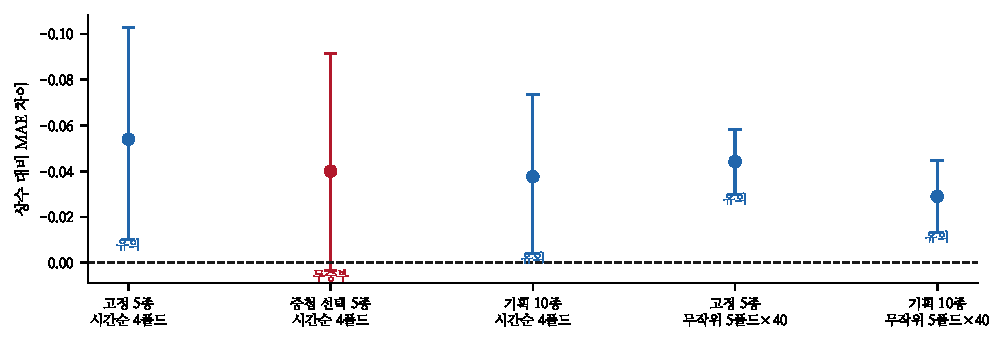
\includegraphics[width=\textwidth]{figs/protocol_gap.pdf}
\caption{같은 다섯 축이 프로토콜에 따라 유의하기도 하고 아니기도 하다. 왼쪽 두 막대가
노트 4와 이 노트의 직접 비교다 --- 선택을 폴드 안으로 넣자 신뢰구간이 0을 넘는다.
오른쪽 두 막대는 무작위 분할 반복 결과로, 다시 0을 넘지 않는다.}
\end{figure}

\claimx{노트 4의 표제 주장 ``다섯 개 속성이 상수를 유의하게 이겼다''를 철회한다.
그 유의성은 선택 편향으로 부풀려진 값이다. 편향을 제거하면 차이는 $-$0.0400이고
신뢰구간이 0을 넘어간다.}{같은 다섯을 미리 고정한 채 새로 수집한 독립 표본에서
검정해 신뢰구간이 0을 넘지 않으면, 이 철회는 과했던 것이 된다.}

\section{살아남은 것: 선택하지 않기}

표에서 눈에 띄는 것은 세 번째 줄이다. 아무것도 고르지 않고 열 개를 전부 넣은 집합이
유의하게 이긴다. 차이의 크기는 중첩 선택보다 작지만($-$0.0376 대 $-$0.0400) 신뢰구간이
훨씬 좁다.

이유는 분산이다. 중첩 선택의 평균 성능은 조금 더 좋지만 폴드마다 다른 다섯을 고르기
때문에 폴드 간 편차가 크다. 선택 자체가 잡음원이 된다. 열 개를 전부 쓰면 어떤 속성이
그 폴드에 안 맞아도 나머지가 흡수한다.

\begin{figure}[t]
\centering
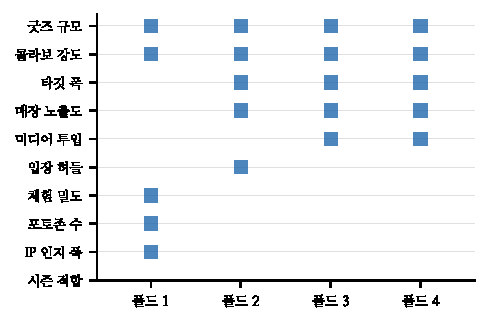
\includegraphics[width=\columnwidth]{figs/sel_instability.pdf}
\caption{폴드마다 다른 다섯을 고른다. 네 폴드 전부에서 뽑힌 것은 굿즈 규모와 콜라보
강도 둘뿐이다. 나머지 여덟 개는 폴드에 따라 들어갔다 나갔다 한다.}
\end{figure}

\paragraph{그리고 하나가 정면으로 어긋난다}
폴드별 선택 결과를 보면 \textbf{콜라보 강도가 네 폴드 전부에서 뽑혔다}. 그런데 노트 4는
콜라보 강도를 IP 인지 폭과 함께 \emph{제거했을 때 오히려 성능이 좋아지는} 두 속성으로
지목했다. 같은 데이터, 같은 절차, 정반대 결론이다.

이 모순은 어느 쪽이 틀렸다는 뜻이 아니라 \emph{둘 다 표본 크기가 감당하지 못하는
판정을 했다}는 뜻이다. n=75, 후보 10개에서 개별 속성의 기여를 순위 매기는 것은
데이터가 지탱하지 못한다.

\claimx{n=75에서 열 개 속성 중 어느 부분집합이 좋은지는 데이터로 결정할 수 없다.
같은 절차가 폴드마다 다른 답을 내고, 노트 4가 해롭다고 지목한 속성을 전 폴드에서
선택한다.}{n을 150 이상으로 늘렸을 때 폴드 간 선택 일치도(자카드)가 0.8을 넘으면
결정 가능해진 것이다. 현재 인접 폴드 간 일치도는 0.4에서 0.6이다.}

\section{그런데 다섯 축은 왜 계속 이기나}

여기서 끝내면 다섯 축은 폐기된다. 그런데 세 번째 실험이 반대 방향을 가리킨다.

시간순 4폴드는 검정 구간이 언제나 최근 데이터이므로 폴드가 넷뿐이고 각 폴드의 검정
표본이 얇다. 신뢰구간이 넓은 것은 당연하다. 시간 제약을 풀고 IP 단위 무작위 5폴드를
서로 다른 난수 40회로 반복하면 표본을 훨씬 촘촘히 쓸 수 있다. 미래 정보를 쓰므로
실전 성능의 상한이지 실전 추정치는 아니지만, \emph{효과의 안정성}을 재는 데는 낫다.

\begin{table}[t]
\centering\tsize
\caption{IP 무작위 5폴드 $\times$ 40회 반복. 시간 순서 제약 없음.}
\begin{tabular}{lrrrr}
\toprule
피처 집합 & 차이 중앙 & 평균 & 표준편차 & 상수를 이긴 비율 \\
\midrule
기획 10종 & $-$0.0290 & $-$0.0282 & 0.0078 & 98\% \\
고정 5종  & $-$0.0442 & $-$0.0420 & 0.0071 & 100\% \\
\bottomrule
\end{tabular}
\end{table}

\begin{figure}[t]
\centering
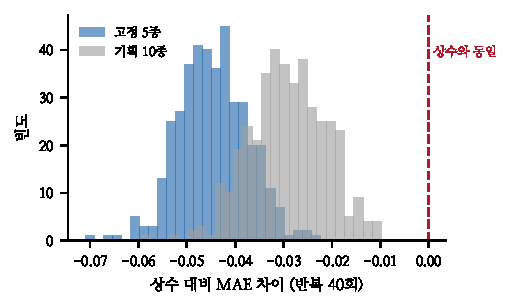
\includegraphics[width=\columnwidth]{figs/repeat_dist.pdf}
\caption{40회 반복의 차이 분포. 고정 다섯 종은 40회 전부 0의 왼쪽에 있다. 열 종보다
분포 전체가 왼쪽으로 밀려 있으며 폭은 비슷하다.}
\end{figure}

고정 다섯 종은 40회 중 40회 상수를 이겼고, 열 종보다 일관되게 더 나았다. 무작위
분할이 관대한 프로토콜이라는 점을 감안해도, 다섯이 열보다 나쁘다는 신호는 어디에도
없다.

\section{세 결과를 화해시키기}

정리하면 이렇다.

\begin{enumerate}[leftmargin=1.3em,itemsep=0.2em]
\item 다섯을 \emph{고정해서} 쓰면 안정적으로 이긴다 (40/40회).
\item 다섯을 \emph{데이터에서 고르게} 하면 이득이 사라진다 (신뢰구간이 0을 넘음).
\item 아무것도 고르지 않고 열을 전부 쓰면 약하지만 이긴다 (신뢰구간이 0을 안 넘음).
\end{enumerate}

1번과 2번이 모순처럼 보이지만 아니다. 두 문장은 서로 다른 것을 말한다.

\begin{quote}\fontsize{9.2}{11}\selectfont
\textbf{그 다섯이 옳은 축인가?} --- 현재 증거로는 그렇다. 고정해 쓰면 반복 검정에서
언제나 이긴다.\\[0.35em]
\textbf{데이터가 그 다섯을 알려줄 수 있나?} --- 아니다. 폴드 안에서 고르게 하면 매번
다른 답이 나오고 이득이 사라진다.
\end{quote}

즉 다섯 축은 \emph{존재하지만 발견 가능하지 않다}. n=75에서 그 다섯이 선택된 경로는
데이터가 아니라 데이터를 본 사람이었고, 그 경로는 재현되지 않는다.

\claimx{다섯 축은 실재할 가능성이 높으나 현재 표본으로는 데이터에서 발견할 수 없다.
따라서 그 다섯을 쓰려면 데이터가 아니라 도메인 이론으로 정당화해야 한다.}{n이 충분히
커진 뒤 순수 데이터 기반 선택이 이 다섯에 수렴하면, ``발견 불가''는 표본 문제였을 뿐
이론적 정당화는 불필요했던 것이 된다.}

\section{파운데이션 모델 설계에 대한 함의}

이 결과는 표본 크기에 관한 기술적 각주가 아니라 아키텍처 결정을 바꾼다.

파운데이션 월드모델의 핵심은 도메인을 가로지르는 공유 표현이다. 팝업, 아이돌 데뷔,
광고 모델, 게임 론칭이 같은 잠재 축 위에 놓여야 전이가 일어난다. 그 공유 축을 어떻게
정할 것인가에 두 갈래가 있다.

\begin{itemize}[leftmargin=1.1em,itemsep=0.15em]
\item \textbf{학습한다}: 다도메인 데이터를 넣고 공유 표현을 학습시킨다. 표준적인
      멀티태스크 접근이다.
\item \textbf{설계한다}: 축을 이론으로 고정하고 데이터는 검증과 보정에만 쓴다.
\end{itemize}

이 노트의 결과는 현재 데이터 규모에서 첫 갈래가 작동하지 않는다고 말한다. 열 개
후보에서 다섯을 고르는 것도 못 하는 표본으로 자유로운 공유 표현을 학습시키면, 학습되는
것은 축이 아니라 잡음이다.

문헌도 같은 방향이다. Standley 등(2020)은 어떤 태스크가 어떤 태스크를 도울지 사전
유사성으로 예측할 수 없고 직접 시험해야만 알 수 있음을 보였으며, 데이터가 5\%로 줄면
해로운 태스크 쌍의 비율이 40\%에서 60\%로 오른다고 보고했다. Maurer 등(2016)의
경계에서 공유 표현 항은 $1/\sqrt{nT}$로, 태스크 고유 항은 $1/\sqrt{n}$로 줄어든다 ---
태스크 수 $T$를 늘리는 것이 공유 항에는 도움이 되지만 태스크당 표본 $n$이 작으면
고유 항이 지배한다. 우리는 $n=75$, $T=1$이다.

\paragraph{그래서 다음 설계는 이렇게 간다}
다섯 축(타깃 폭, 매장 노출도, 입장 허들, 미디어 투입, 굿즈 규모)을 학습 대상이 아니라
\emph{아키텍처의 고정 구조}로 놓는다. 신경망의 첫 층을 이 다섯 축에 해당하는 슬롯으로
고정하고, 도메인별 인코더가 자기 문서를 이 다섯 슬롯에 사상하도록 학습시킨다. 축
자체는 데이터가 바꾸지 못한다. 데이터가 하는 일은 각 도메인의 원자료를 다섯 슬롯으로
번역하는 함수를 배우는 것뿐이다.

이 구조는 표본이 작을 때 유리하다. 자유도가 축 발견에 쓰이지 않고 전부 사상 함수에
쓰인다. 그리고 반증 가능하다 --- 아이돌 도메인 라벨을 확보해 같은 다섯 축을 태깅했을 때
전이가 일어나면 축이 도메인 불변이라는 증거이고, 일어나지 않으면 축은 팝업 국소적이다.

\section{한계}

\begin{itemize}[leftmargin=1.1em,itemsep=0.15em]
\item 무작위 5폴드 반복은 시간 순서를 쓰지 않는다. 실전 성능이 아니라 상한이며,
      안정성 판정에만 쓸 수 있다.
\item ``다섯이 옳다''는 결론은 여전히 이 75건에서 그 다섯이 골라졌다는 사실에
      의존한다. 완전히 독립적인 확증은 새 표본에서만 나온다.
\item 시간순 폴드가 넷뿐이라 짝지은 부트스트랩의 유효 표본이 작다. 신뢰구간 자체가
      넓게 나오는 구조적 이유이며, 유의하지 않음이 효과 없음을 뜻하지 않는다.
\item 열 개 서수 속성은 사람이 매긴 것이고 평정자 간 일치도를 아직 재지 않았다.
      속성 자체의 신뢰도가 성능 상한을 깎고 있을 수 있다.
\end{itemize}

\section{다음}

\begin{enumerate}[leftmargin=1.3em,itemsep=0.15em]
\item 열 개 서수 속성의 평정자 간 일치도 측정 --- 잡음 상한을 먼저 안다.
\item 아이돌 도메인 라벨 확보 후 같은 다섯 축 태깅, 전이 검정. 파운데이션 가설의
      첫 직접 시험이다.
\item 다섯 슬롯 고정 구조의 최소 신경망 구현과 GBDT 대비 검정.
\item n=150 도달 시 폴드 간 선택 일치도 재측정 --- 발견 가능성이 표본 문제였는지 확인.
\end{enumerate}

\vspace{0.6em}
\hrule height 0.3pt
\vspace{0.5em}
{\footnotesize
\textbf{참고문헌}\\[0.3em]
Ben-David, S. et al. (2010). A theory of learning from different domains.
\emph{Machine Learning}, 79(1--2), 151--175.\\[0.15em]
Maurer, A., Pontil, M., Romera-Paredes, B. (2016). The benefit of multitask
representation learning. \emph{JMLR}, 17(81), 1--32.\\[0.15em]
Riley, R. D. et al. (2019). Minimum sample size for developing a multivariable
prediction model. \emph{Statistics in Medicine}, 38(7), 1262--1275.\\[0.15em]
Standley, T. et al. (2020). Which tasks should be learned together in multi-task
learning? \emph{ICML 2020}, 9120--9132.\\[0.15em]
Varma, S., Simon, R. (2006). Bias in error estimation when using cross-validation
for model selection. \emph{BMC Bioinformatics}, 7, 91.
}

\end{document}
